\chapter{Design}
Within this section, I will explain how and why I chose the Software Architecture I did, and what tools I used to develop Inhale.\\

As all of the datasets used with Inhale are geographical datasets. This means they all have a location attribute, so it is imperative that they are displayed on a map; trying to make any sense of a geographical dataset without seeing it on a familiar map is nearly impossible.\\

\subsection{ArcGIS by Esri}

ArcGIS is an incredibly powerful contextual tool for mapping and spatial reasoning, it is available both online and to download as a desktop application. Its features are so well made that I initially thought that using some form of this software would be the only viable solution. It allows you to produce aesthetically pleasing, user-friendly maps with very few lines of code. It  also provides a mass of data processing tools, including hotspots analysis and data correlation.\\

\begin{figure}[H]
\begin{center}
\includegraphics[width=0.6\textwidth]{esridesktop}
\label{fig:esri}
\caption{An example of what Esri's ArcGIS can do \cite{esridesktop}}
\end{center}
\end{figure}

Despite its efficiency, I chose not to go with ArcGIS due to its very high licensing cost. I wanted to implement my own algorithms, using ArcGIS would not leave me with much to implement in terms of algorithms, and after all, this is a computer science project. Ultimately, I can see how ArcGIS could be incredibly useful for businesses and marketing purposes, but it's not fit to be used in a project where one of the main motivations is to improve my programming skills and gain experience with new technologies.\\

\subsection{Desktop Mapping Tools}

There are various desktop based mapping tools available, including open source options that have a wide variety of features. The main issue with this style of mapping software is it's lack of expandability, accessibility and familiarity.\\

Although tools such as MapSphere allow you to make third party plugins to expand the standard application with your own features, the features you're given access to when developing those plugins is quite limited. I want the scope to be able to implement whatever I want.\\

When creating a desktop application, you're instantly cutting down your potential users. Not everyone wants to download an application, it feels too heavy and sluggish for modern users when we can access perfectly able maps from our pockets in the form of smartphone apps and websites. I wanted Inhale to be familiar to the user, I wanted to use controls people are familiar with from their everyday use of Google Maps, Waze etc. All of the free desktop applications I explored felt very dated, so it was important to me to avoid making the same mistakes.\\

\subsection{Google Maps}

After discounting ArcGIS and various desktop mapping tools, I was aiming more towards a solution involving a more dynamic mapping provider. Google have an API that allows developers to implement their own features, toolbars and map tiles. The API can provide maps on various platforms from Android, iOS, JavaScript and more.\\

The biggest incentive towards Google Maps is their Places API, it allows the user to search for establishments, geographic locations, or prominent points of interest in a well-defined area around a point \cite{googlePlaces}. This would be incredibly useful for Inhale, as once a hotspot is identified you can search for nearby places that may be contributing to the symptoms in that area. The only problem here is that it's very difficult to implement a general approach that works for all locations to get nearby places that might have an effect on allergy symptoms. Google organise places by type, however the types are aimed more towards general public use. They're in categories such as art gallery, bakery, bank, pharmacy, hospital. Whilst it could be argued that you could count the number of commercial premises nearby to make an estimation of commercial pollution, I don't believe this is enough to provide any sort of answer to why allergies are so prevalent in any given area.\\

Google Map's main downfall is the lack of expandability and features compared to other mapping options. If Google ever increases the number of categories for Places, or includes more general options for types such as industrial or factory then it could absolutely be considered as the best option.\\

\subsection{Leaflet}

Leaflet is a JavaScript library for mobile-friendly interactive apps \cite{leaflet}. Leaflet is comparable to Google Maps in that it has many of the same features and uses. Leaflet is open source, has many third party plugins with a thriving community contributing daily towards building a versatile dynamic mapping tool.\\

Leaflet is the most customisable of all the options investigated so far. It allowed me more freedom to develop what I want in terms of behind the scenes processing, and make my map look better, see \ref{fig:leafletexf} for and example of what you can do with Leaflet. The main drawbacks are that it does not provide any spatial reasoning tools, nor does it have any built-in place recognition like Google.\\

\begin{figure}[H]
\begin{center}
\includegraphics[width=0.6\textwidth]{leafletexp}
\label{fig:leafletexf}
\caption{Hexbins using Leaflet}
\end{center}
\end{figure}

One particular third party plugin that drew me towards Leaflet was heatmap.js. I believe heatmaps are the best way to present the results of a hotspot identification algorithm. After testing the built-in Google Maps heatmap, I was disappointed with both the speed and custom options available. Leaflet with heatmap.js outperformed Google in this respect, this is what convinced me to use Leaflet as my mapping tool of choice.

\section{Software Environment}

My environment options for Inhale were to make a Desktop Application for either Windows or MacOS, a mobile app or a web application.\\

I decided against making a desktop app for any platform as by going with this route it limits the number of users immediately. Whilst the last two versions of Windows make up around 65\% of the Desktop market, that leaves a potential 35\% of users that are completely unable to use my software \cite{windows}. As this project is likely to be shown to potential employers, it would be preferable to have it on a platform that is easier to setup and present. Furthermore, I want to avoid compatibility issues and requiring updates to run with new .NET versions for example.\\

Although a mobile application on either main platform was a strong contender. Android has recently overtaken Windows as the most popular operating system for Internet users, which means that I wouldn't be ruling out as many users from using my application \cite{android}. The decision to avoid mobile applications for this project was mainly due to wanting the project to be designed with research usage in mind. These users would likely want to use the more advanced features of Inhale which would require more screen real estate to get the benefits. Finally, I want users to be able to upload their own datasets. As research users don't generally store their datasets on their mobiles. It makes sense to build this project in a standard web environment.\\

Leaflet was chosen because it can be used in a web format, it is very customisable, and it has a lively community contributing to features all the time. It would be easy to add necessary features further down the line.

\section{Development Tools}

Tableau is a desktop data processing tool that pride themselves on the fast processing of big data. They offer a massive amount of data processing tools, including visualising map data very quickly and easily. Thanks to their free student license, this ease of viewing geographical datasets made it my first choice of software when exploring new datasets. It allowed me to rule out sets very quickly without wasting time, allowing me more development time.\\

\begin{figure}[H]
\begin{center}
\includegraphics[width=1\textwidth]{tab}
\label{fig:tabf}
\caption{Tableau, an excellent data processing tool}
\end{center}
\end{figure}

Google's development tools included in their Chrome browser was very useful troubleshooting and debugging during development. The Elements tab was used for designing and tweaking HTML and CSS. The Network and Console tabs were used for testing, debugging during run time and timing the efficiency of certain pieces of code.\\

\begin{figure}[H]
\begin{center}
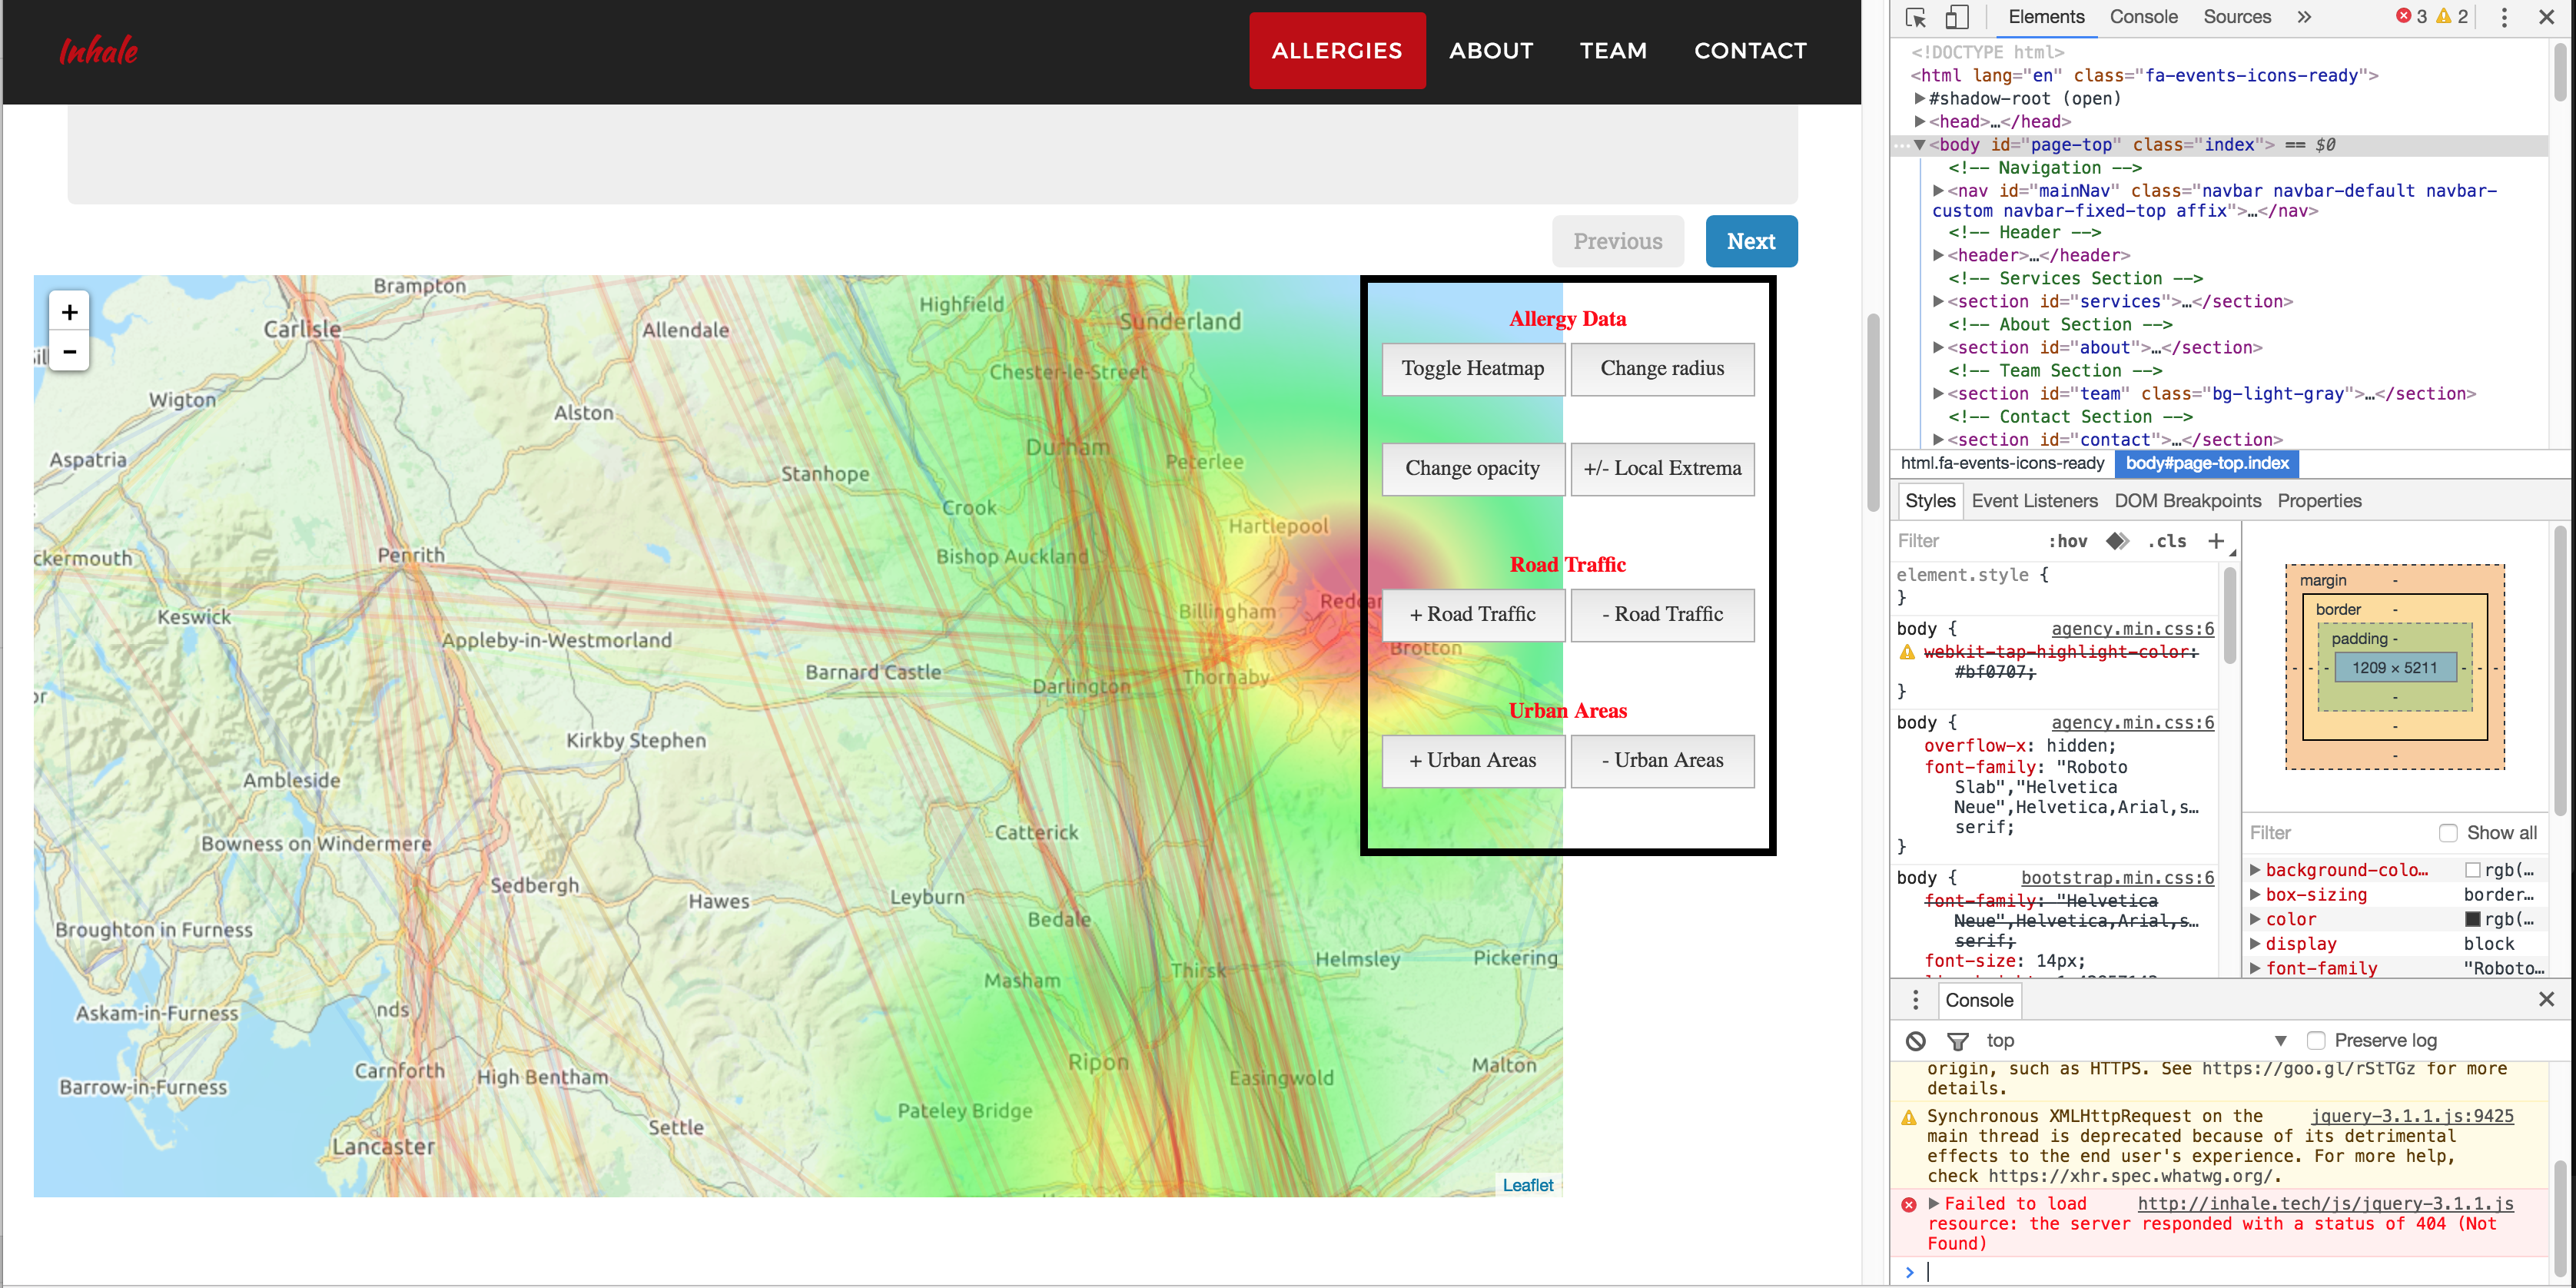
\includegraphics[width=1\textwidth]{devtools}
\label{fig:devtoolsf}
\caption{Google Chrome's development tools in action}
\end{center}
\end{figure}